Como mencionado anteriormente, o desafio anual \emph{ImageNet Large Scale Visual Recognition Challenge} (ILSVRC) têm tido um papel protagonista no desenvolvimento de soluções em DL, pois têm promovido um contexto para proposição e comparação de algumas das arquiteturas de CNNs mais bem sucedidas para problemas de detecção de objetos e classificação de imagens em larga escala \cite{ILSVRC}.

Entre os anos de 2010 e 2014, os resultados alcançados pelo ILSVRC melhoraram significativamente nas três categorias existentes. Os desempenhos alcançados neste cenário são mostrados no gráfico da Figura \ref{fig:ilsvrc} de acordo com a métrica utilizada em cada categoria \cite{ILSVRC}.   

\begin{figure}[h]
	\centering
	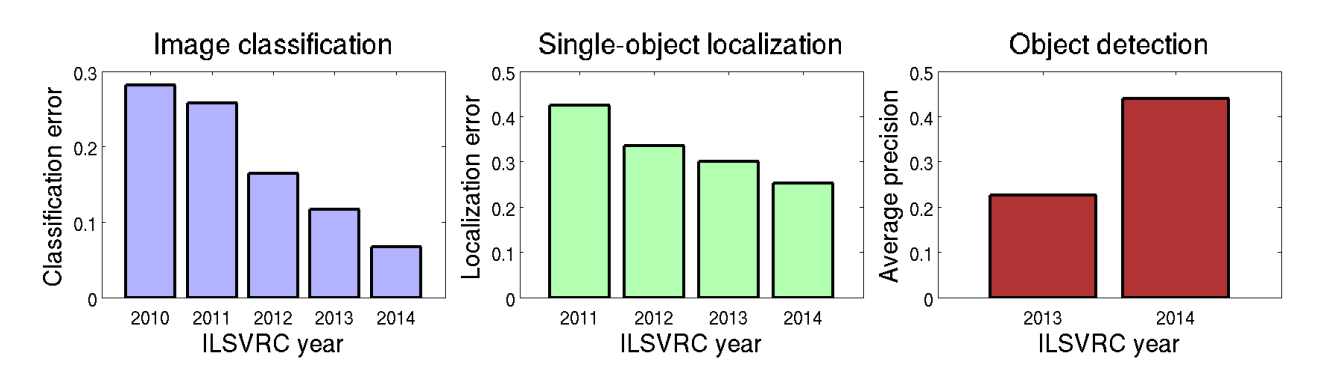
\includegraphics[width=1\textwidth]{./img/ilsvrc}
	\caption{Desempenhos alcançados do ILSVRC entre os anos de 2010 e 2014.}
	\label{fig:ilsvrc}
\end{figure}

Embora os conceitos das camadas de uma CNN estejam bem estabelecidos e sejam de conhecimento geral, nem sempre é uma tarefa fácil propor uma rede neural deste tipo para um determinado cenário. Assim, uma consequência positiva da realização do ILSVRC é promover a difusão das arquiteturas de destaque na competição, as quais passam ser conhecidas e adaptadas pela comunidade acadêmica e tecnológica na resolução de diversos outros problemas. Considerando esta importância e potencial de aproveitamento de soluções, a seguir são apresentadas algumas destas arquiteturas canônicas.


\paragraph{LeNet} Yann le Cun desenvolveu, em 1990, uma das primeiras arquiteturas utilizadas para o reconhecimento de dígitos manuscritos, a LeNet. Vencedora do ILSVRC 2010, esta arquitetura é composta por três camadas convolucionais alternadas com camadas de \textit{pooling} seguidas de duas FCLs conforme representado na Figura \ref{img:lenet} \cite{ref:sewak,ref:khan}.

\begin{figure}[!ht]
	\centering
	\caption{Arquitetura LeNet de CNN. Fonte: \cite{ref:khan}.}
	\label{img:lenet}
	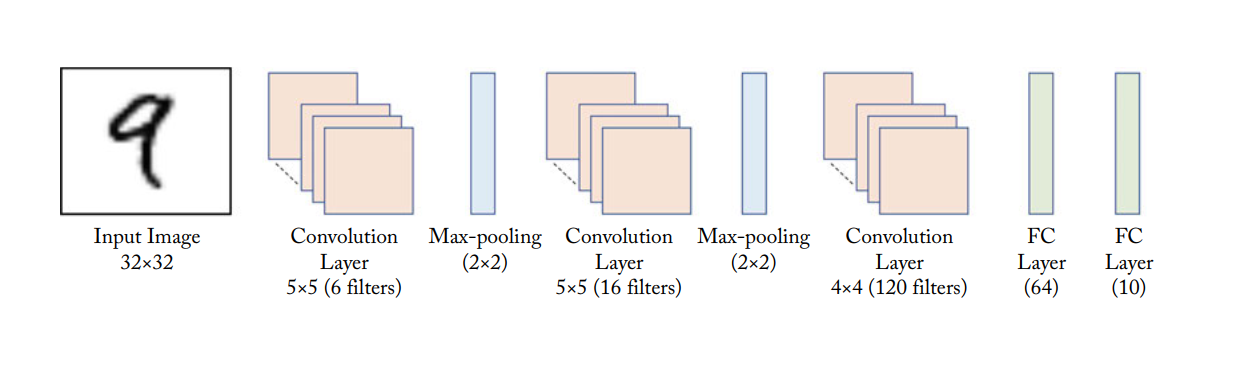
\includegraphics[width=1\textwidth]{./img/lenet}
\end{figure}


\paragraph{AlexNet} Em 2012, a vencedora do ILSVRC foi a arquitetura proposta por Alex Krizhevsky, conhecida como AlexNet, ilustrada na Figura \ref{img:alexnet}. A AlexNet é mais profunda e uma versão muito mais ampla da arquitetura LeNet \cite{ref:satapathy}. A principal diferença entre a AlexNet e as CNNs predecessoras é a sua maior profundidade, que lida muito bem com sua grande quantidade de parâmetros, além da utilização de artifícios como \textit{dropout} e \textit{data augmentation}. As cinco primeiras camadas da arquitetura AlexNet são camadas de convolução e \textit{pooling} alternadas de forma similar à LeNet, porém, seguem-se mais três camadas, duas convolucionais e uma de\textit{pooling}. As últimas camadas são FCL, mas além destas existem camadas \textit{dropout} que ajudam à reduzir \textit{overfiting} \cite{ref:khan}.

\begin{figure}[!ht]
	\centering
	\caption{Arquitetura da AlexNet. Fonte: \cite{ref:khan}.}
	\label{img:alexnet}
	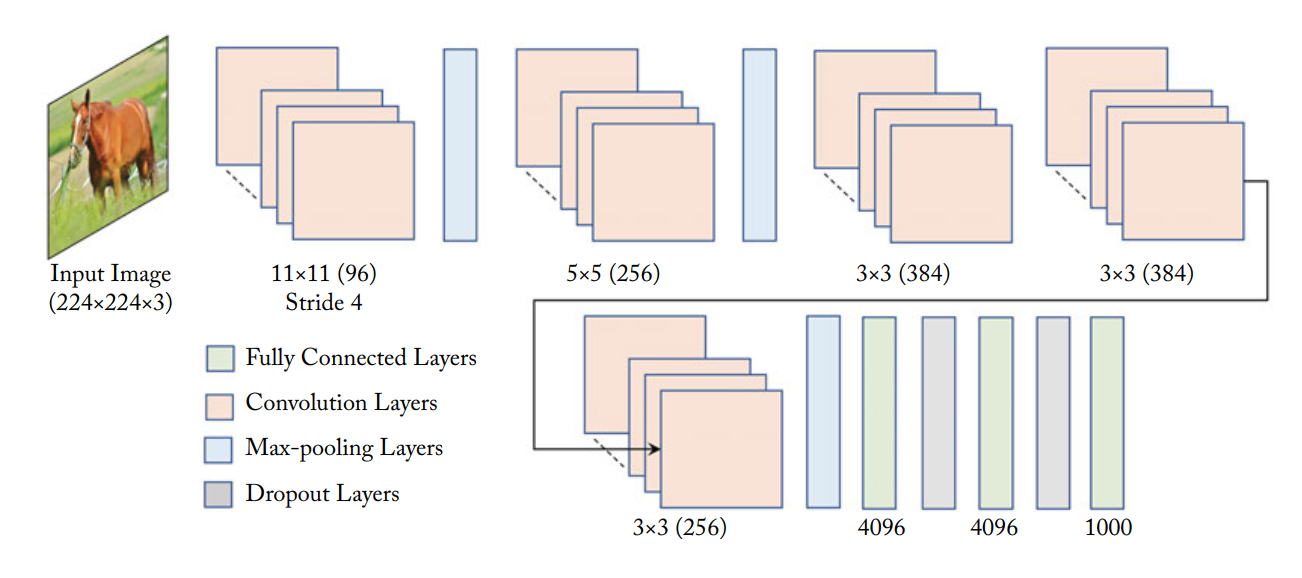
\includegraphics[width=1\textwidth]{./img/alexnet}
\end{figure}

\paragraph{VGGNet} A arquitetura VGGNet é uma das arquiteturas mais populares desde sua criação em 2014, apesar de não ter sido a vencedora do ILSVRC realizado no respectivo ano. A razão de sua popularidade se dá especialmente em virtude do uso de pequenos filtros de convolução, diminuindo o número de parâmetros ajustáveis e, por conseguinte, aumentando a eficiência do treinamento. A arquitetura VGGNet usa estritamente fitros de convolução de dimensão $3 \times 3$ combinados com camadas de \textit{pooling} para extração de características e um conjunto de três FCLs. Além das camadas de convolução, \textit{pooling} e das camadas conectadas, esta arquitetura também possui as camadas \textit{dropout} como pode ser observado na Figura \ref{img:vggnet} \cite{ref:khan}.

\begin{figure}[!ht]
	\centering
	\caption{Arquitetura VGGNet. Fonte: \cite{ref:khan}.}
	\label{img:vggnet}
	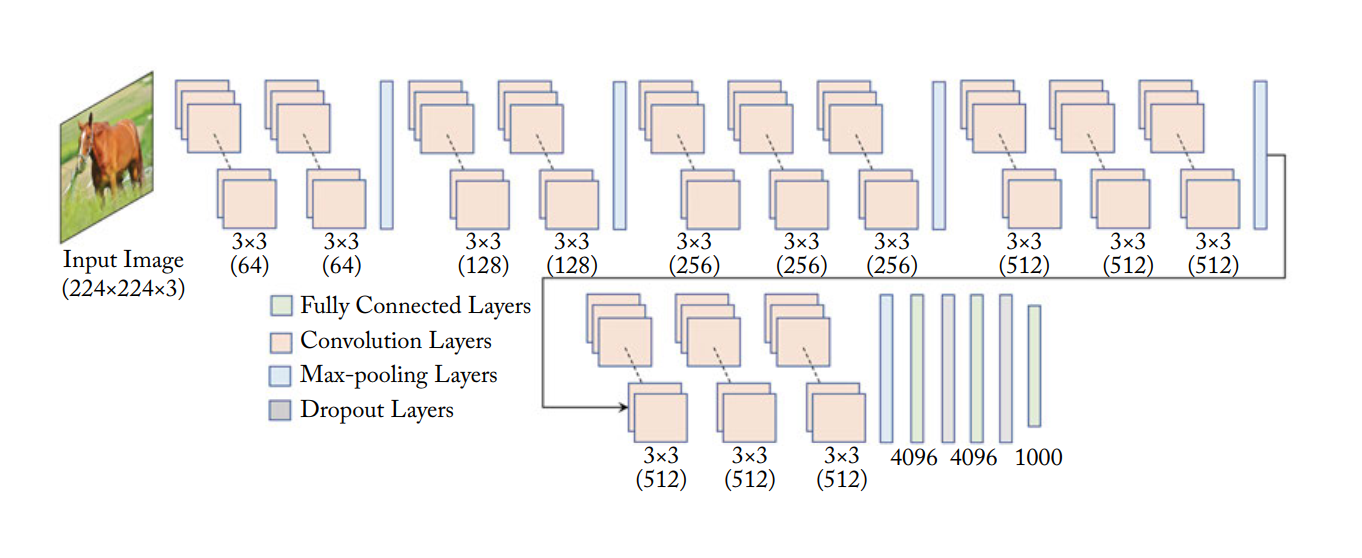
\includegraphics[width=1\textwidth]{./img/vggnet}

\end{figure}

\paragraph{GoogLeNet} Desenvolvida pela empresa Google e vencedora do ILSVRC 2014, a arquitetura GoogLeNet possui $22$ camadas baseadas em um módulo elementar chamado \emph{Inception Module}. O processamento desses módulos ocorre de forma paralela, diferentemente do processamento sequencial das arquiteturas discutidas anteriormente. A ideia central da arquitetura GoogLeNet é paralelizar os módulos e combinar as características da saída sem se preocupar com as funções individuais de cada camada. No entanto, essa abordagem resulta em um mapa de características com muitos elementos, mas para contornar este problema, após a execução do primeiro módulo, a rede realiza uma redução de dimensionalidade utilizando uma FCL antes de continuar o processo de treinamento \cite{ref:khan}. A representação da arquitetura GoogLeNet encontra-se na Figura \ref{img:googlenet}.

\begin{figure}[!ht]
	\centering
	\caption{Arquitetura GoogLeNet. Fonte: \cite{ref:khan}.}
	\label{img:googlenet}
	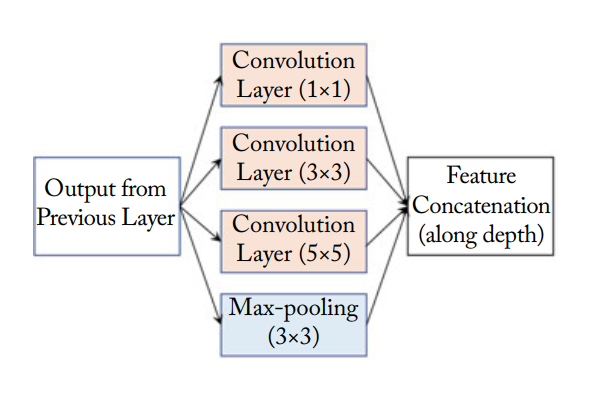
\includegraphics[width=0.6\textwidth]{./img/googlenet}

\end{figure}
